\chapter{CPU}

\section{流水线结构}

\subsection{总体架构}

CPU采用双发射顺序执行,共有10级流水。整体的流水线结构如图 \ref{fig:cpu-pipeline} 所示。其中为了能够得到较高的频率,指令和数据Cache均采用3级流水。为了解决访存周期过长而导致的访存暂停过多,我们动态地判断指令的执行时间,允许指令在操作数没有准备好时就发射,并且在操作数准备好时再执行。流水线各个阶段的功能会根据指令类型和数据相关情况动态变化。

各个阶段的功能大致如下:
\begin{itemize}
    \item \textbf{取指1} 计算当前PC,发送请求给指令Cache。
    \item \textbf{取指2} 指令Cache读取数据。
    \item \textbf{取指3} 对指令进行简单译码,进行简单的分支解析,将指令包放入FIFO。
    \item \textbf{译码/发射}\, 从FIFO获取指令包,进行译码并且决定是否发射。
    \item \textbf{读操作数}\, 从寄存器堆以及数据旁路读取操作数。
    \item \textbf{执行}\, 执行指令。读取存储指令的数据。
    \item \textbf{访存1/延迟读操作数}\,  向数据Cache发送访存请求。同时处理异常,对于延迟执行的指令进行操作数读取。
    \item \textbf{访存2/延迟执行}\, 数据Cache计算数据。延迟执行的指令在此时执行。
    \item \textbf{访存3}\, 读取访存结果。
    \item \textbf{写回}\, 写回数据到寄存器堆。
\end{itemize}

\begin{landscape}
\begin{figure}[htbp]
	\centering
	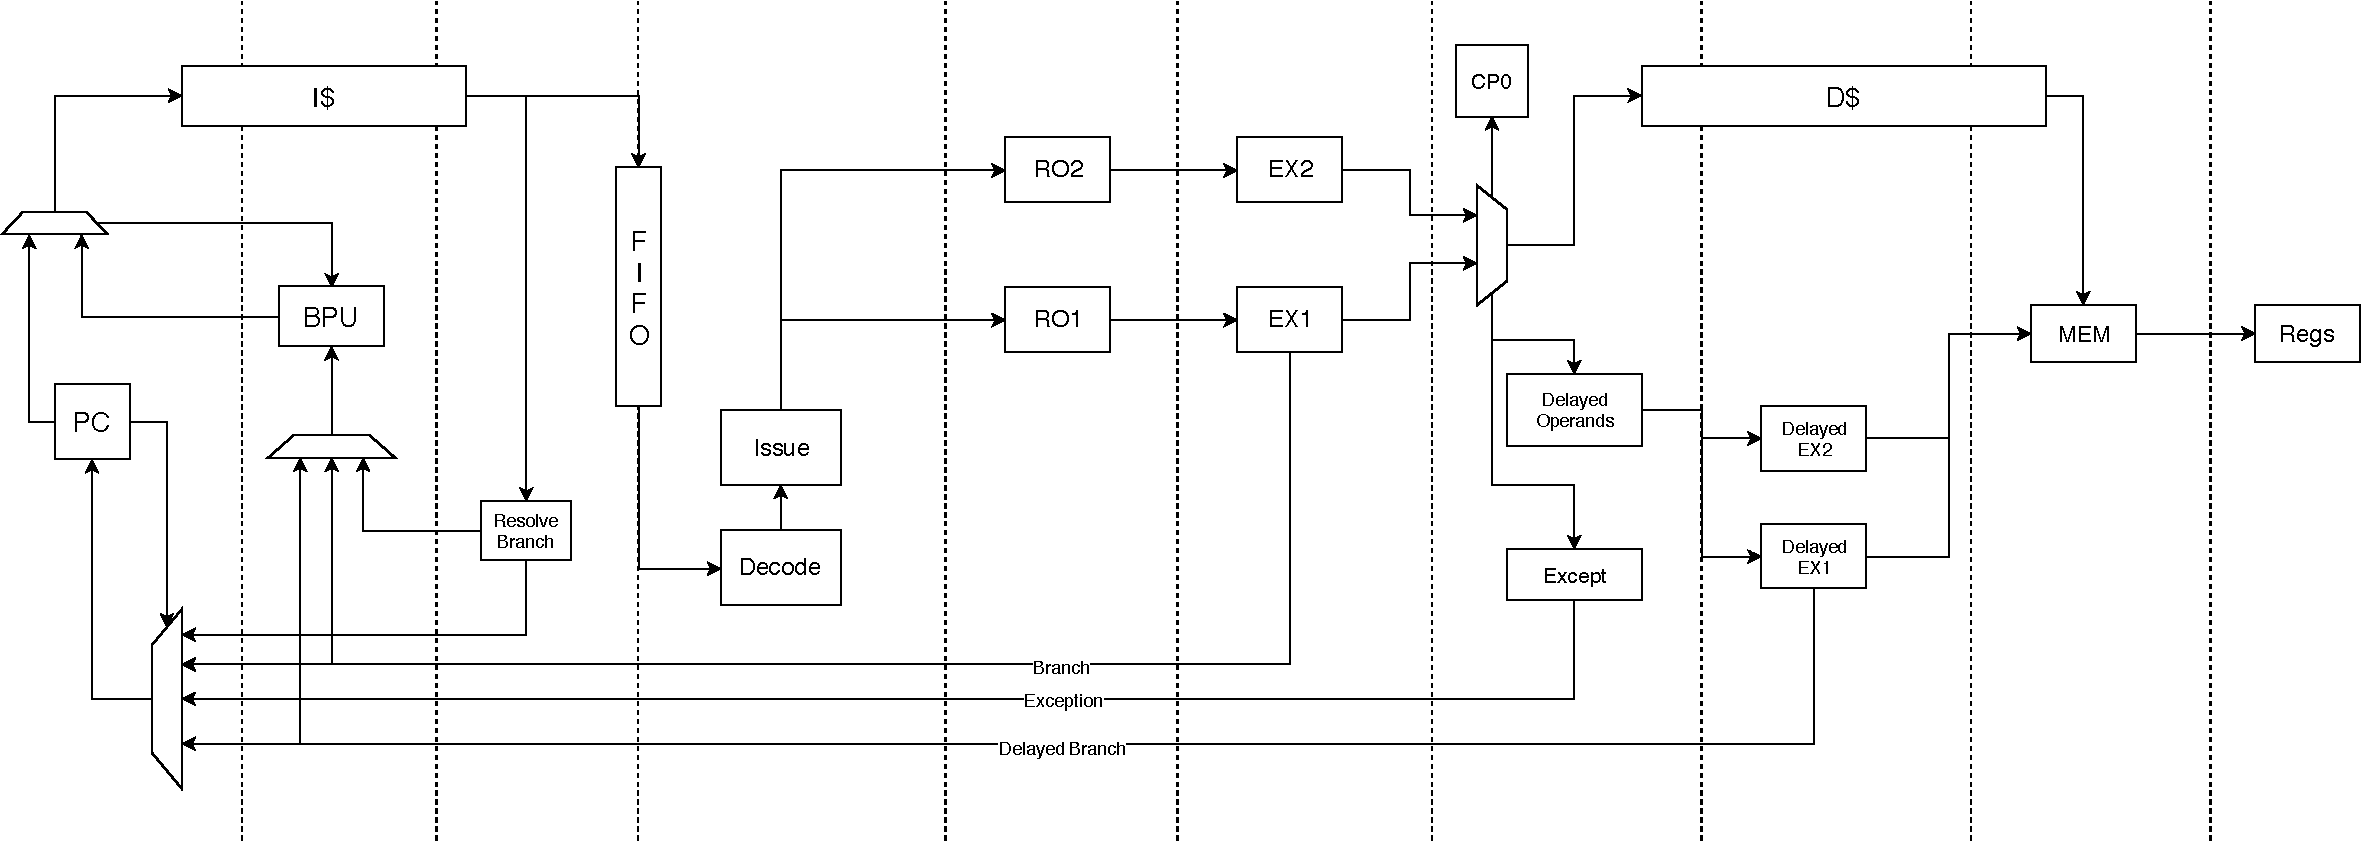
\includegraphics[width=\linewidth]{cpu-design.pdf}
	\caption{CPU流水线结构}
	\label{fig:cpu-pipeline}
\end{figure}
\end{landscape}

\subsection{取指阶段}
取指阶段共有3级流水,最后得到的指令会放入指令FIFO。在此3阶段中同时会进行分支预测,同时能够保证在分支命中的情况下放入FIFO的指令流就是所需要执行的指令流。分支预测失败会刷新指令FIFO,该信息由执行单元生成。

分支预测采用传统的2比特分支预测,BTB和BHT采用BRAM实现,延迟为一个周期。

取指的第一个阶段,会计算取指的地址并且发送给Cache,同时计算下一个PC的值。

取指的第二个阶段,会对下一个阶段需要放入FIFO的指令包的一部分内容进行计算。

取指的第三个阶段,会对得到的指令进行简单的译码,判断是否为分支同时反馈给分支预测和PC生成器。如果将非分支指令预测为分支,那么及时进行流水线刷新。此阶段还会将指令包放入指令FIFO,至多会有3条指令被放入(即第二条指令是分支,并且延迟槽和分支在同一个Cache行中)。

当前周期所需要取指的地址通过当前PC和BTB/BHT得到的分支信息得到,下一个周期的PC受到当前PC,分支预测信息,指令FIFO是否满,异常请求和执行阶段所解析的分支信息控制。如果指令FIFO满则会丢弃当前数据并且重新在对应为止取指。

为了支持多发射流水线,指令Cache要求地址按照8字节对齐,每次会返回64位的数据,另外如果随后的64位数据仍然在Cache行内,也会将其返回,这是为了更快地处理延迟槽。由于MIPS具有延迟槽机制,我们在分支预测跳转之后还需要将延迟槽也放入指令FIFO。为了尽量获取更多的指令,如果指令Cache返回的64或者128位数据中有延迟槽,那么当前就可以直接取分支目标的指令,否则需要取延迟槽指令。

\subsection{译码和发射阶段}
译码和发射均在流水线的第4个阶段。译码器会从指令FIFO中获取对应信息,并且进行译码。

发射阶段较为复杂,其共分为如下几种情况
\begin{enumerate}
    \item 由于我们的流水线设计中仅有一个乘法器和除法器,乘除指令一个周期内最多只能发射一条。另外,为了设计简便,CP0相关指令一个周期内也最多只能发射一条。除此之外,由于只有一个访存单元,访存指令在一个周期最多也只发射一条。
    \item 如果一个发射包内两条指令存在数据相关,那么只发射第一条指令。
    \item 分支指令必须和延迟槽一起发射,如果延迟槽没有取到则需要暂停,如果分支指令是发射包第二条指令则不能发射。
\end{enumerate}

由于访存结果在流水线第9个阶段才能得到,如果在译码阶段直接读操作数则访存相关需要3个周期的暂停。为了更好地处理访存相关,我们进行部分指令的延迟执行。具体来说,如果指令在译码阶段后不会产生异常(例如AND,XOR,ADDU等),我们可以将这类指令的操作数读取延迟到访存的第一阶段,执行延迟到访存的第二阶段。这样访存相关的暂停最好可以缩短到一个周期。更进一步,我们还可以将分支指令也推迟到这个阶段。但是由于分支有可能预测失败,我们需要能够撤销其后的指令。幸运的是,访存请求的提交和异常的触发都是在访存第一阶段,而分支指令的解析是在访存第二阶段,并且其延迟槽不会有异常。这样恰好可以在解析到分支预测失败时刷新流水线,使得其后的指令不会改变处理器状态。

当然,如果指令不能延迟执行,那么仍然需要暂停到操作数均可用为止。此时的访存相关还要考虑正在延迟执行的指令而不仅仅是访存指令。

总的来说,在发射阶段需要暂停的情况大致如下:
\begin{enumerate}
    \item 指令无法延迟执行,并且操作数没有准备好。这包含访存指令数据没有准备好,以及延迟执行的指令结果没有准备好。
    \item 指令可以延迟执行,但是在执行阶段有访存指令。这是真正的无法消除的访存相关。
    \item 分支指令但是延迟槽还不在FIFO中。
    \item 执行阶段正在执行特权指令。这是由于CP0的设计原因。
    \item 流水线上存在非MFC0和MTC0的特权指令,这是为了解决可能的CP0冒险。
\end{enumerate}

\subsection{读操作数阶段}
指令所需要的两个操作数在第5个阶段从寄存器堆和数据旁路读取。对于延迟执行的指令,此时读取的操作数可能是无效的,会在之后再次读取。对于存储指令,存储的数据可能是无效的,会在执行阶段再次读取。

\subsection{执行阶段}
执行阶段是流水线的第6个阶段。此阶段会生成指令的结果,同时计算异常请求,计算访存地址。

对于内存写指令(如SW、SC等)会在此阶段读取需要写的数据。对于多周期指令,在计算完前会生成一个暂停信号。流水线仅有一个乘法和除法单元。

\subsection{访存阶段}
访存阶段是流水线的第7, 8, 9阶段,在第7阶段将访存请求发送给数据Cache,在第9个阶段可以得到访存结果。

该阶段和延迟执行阶段是重叠的。

\subsection{延迟执行阶段}
大部分指令都是在译码阶段读取操作数,在执行阶段计算结果。如果指令之间存在访存相关,并且指令是分支或者不会在执行阶段出现异常,那么其可以在流水线第7阶段读取操作数,其后一个阶段计算结果。如果是分支指令则会生成分支结果反馈给分支预测器。

该阶段和访存阶段是重叠的。

\subsection{写回阶段}
此阶段写回寄存器请求,是流水线的最后一个阶段。
\section{指令集}
下方按照功能划分列举了CPU所支持的MIPS指令,各条指令的具体编码以及功能在MIPS文档中有详细的描述。
\begin{itemize}
	\item \textbf{自陷指令} TGE, TEGU, TLT, TLTU, TEQ, TNE, TGEI, TGEIU, TLTI, TLTIU, TEQI, TNEI
	\item \textbf{分支指令} BLTZ, BGEZ, BLTZAL, BGEZAL, BEQ, BNE, BLEZ, BGTZ, JR, JALR, J, JAL
	\item \textbf{逻辑指令} AND, OR, XOR, ANDI, ORI, XORI, NOR, SLL, SRL, SRA, SLLV, SRLV, SRAV
	\item \textbf{算术指令} ADD, ADDU, SUB, SUBU, ADDI, ADDIU, MUL, MULT, MULTU, DIV, DIVU, MADD, MADDU, MSUB, MSUBU, CLO, CLZ
	\item \textbf{访存指令} SB, SH, SW, SWL, SWR, LB, LH, LWL, LWR, LW, LBU, LHU, LL, SC
	\item \textbf{特权指令} CACHE, SYSCALL, BREAK, TLBR, TLBWI, TLBWR, TLBP, ERET, MTC0, MFC0
	\item \textbf{条件移动指令} SLT, SLTU, SLTI, SLTIU, MOVN, MOVZ
	\item \textbf{无条件移动指令} LUI, SLT, SLTU, MFHI, MFLO, MTHI, MTLO 
\end{itemize}

\section{协处理器0}
CP0是MIPS规范中必要的一个协处理器,它提供了操作系统所必须的功能抽象,例如异常处理、内存管理和资源访问控制等。

在CP0中有多个32位寄存器,各个寄存器均通过MTC0和MFC0读写。另外,诸如TLBWI、TLBWR和TLBP等特权指令还有异常的发生也有可能会影响其值。

表\ref{table:required_cp0_registers}中列出了必须实现的CP0寄存器。

\begin{table}[!htbp]
    \centering
    \caption{必要的CP0寄存器}
    \label{table:required_cp0_registers}
    \begin{tabular}{|r|l|l|}
    \hline
    \textbf{编号} & \textbf{名称} & \textbf{功能}  \\ \hline
	8 & BadVAddr & 最近发生的与地址相关的异常所对应的地址 \\ \hline
	9 & Count & 计数器 \\ \hline
	11 & Compare & 计时中断控制器 \\ \hline
	12 & Status & 处理器状态及控制 \\ \hline
	13 & Cause & 上一次异常的原因 \\ \hline
	14 & EPC & 上一次异常发生的地址 \\ \hline
	15 & PRId & 处理器版本和标识符 \\ \hline
	16 & Config0 & 处理器配置 \\ \hline
	30 & ErrorEPC & 上一次异常发生的地址 \\ \hline
    \end{tabular}
\end{table}

为了实现TLB MMU的功能,还需要表\ref{table:mmu_cp0_registers}中所列出的寄存器。

\begin{table}[!htbp]
    \centering
    \caption{MMU所需要的CP0寄存器}
    \label{table:mmu_cp0_registers}
    \begin{tabular}{|r|l|l|}
    \hline
    \textbf{编号} & \textbf{名称} & \textbf{功能}  \\ \hline
	0 & Index & TLB数组的索引 \\ \hline
	1 & Random & 随机数 \\ \hline
	2 & EntryLo0 & TLB项的低位 \\ \hline
	3 & EntryLo1 & TLB项的低位 \\ \hline
	4 & Context & 指向内存中页表入口的指针 \\ \hline
	5 & PageMask & 控制TLB的虚拟页大小 \\ \hline
	6 & Wired & 控制TLB中固定的页数 \\ \hline
	10 & EntryHi & TLB项的高位 \\ \hline
    \end{tabular}
\end{table}

同时,为了支持自定义异常向量,还需要额外实现一个MIPS 32 Rev 2 中的 EBase寄存器。

\section{中断和异常}
\subsection{中断}
MIPS的中断一共有8个,从0开始编号。其中0号中断和1号中断是软件中断,由软件设置Cause寄存器中的对应位来触发。其余6个中断为硬件中断,由外部硬件触发。在实现中,由Count/Compare寄存器组合而成的定时中断的中断号为7。

如果该中断满足触发条件则会触发异常并且进入中断处理程序。中断的触发要求如下条件全部满足:
\begin{enumerate}
	\item \texttt{Status}寄存器中对应的中断被打开;
	\item 全局中断使能,即\texttt{Status.IE}为1;
	\item 当前不在异常处理程序中,即\texttt{Status.EXL}和\texttt{Status.ERL}为0。
\end{enumerate}

\subsection{异常}
MIPS的异常是“精确异常”,也就是在异常发生前的指令都会执行完毕,异常发生之后的指令不会继续执行。在异常发生时,CPU会跳转到对应的异常向量处执行异常处理代码并设置CP0中对应的寄存器记录异常的原因和一些额外的信息,同时还会进入Kernel Mode。处理异常代码的异常向量由“基地址+偏移”来决定,偏移是根据异常来确定的,基地址是由CP0的EBase寄存器决定。

在我们的实现中,在流水的各个阶段产生了异常,不会马上触发,而是被记录下来,顺着流水直到MEM阶段完成后再进行触发。同时,还会考虑双发射两条流水线,优先触发第一条流水线的异常。特别地,异常返回指令ERET被实现为一种特殊的异常,保留到MEM阶段触发。

需要支持的异常在表\ref{table:main-exception}中列出。

\begin{table}[htbp]
	\centering
	\caption{主要支持的异常}
	\label{table:main-exception}
	\begin{tabular}{|c|c|c|c|} \hline
		\textbf{异常简称} & \textbf{异常说明} & 	\textbf{异常简称} & \textbf{异常说明} \\ \hline
		Int & 中断   & Sys & 系统调用             \\ \hline
		Mod & TLB修改异常 & 	Bp & 断点  \\ \hline
		TLBL & TLB Load异常 & 	RI & 保留指令 \\ \hline
		TLBS & TLB Store异常 & 	CpU & 协处理器不可用 \\ \hline
		AdEL & 地址Load异常 & Ov & 算术溢出\\ \hline
		AdES & 地址Store异常 & 	Tr & 自陷异常 \\ \hline
	\end{tabular}
\end{table}
\section{内存管理}
MIPS为操作系统的内存管理提供了较为简单的支持,虚拟地址通过MMU转换为物理地址。MIPS标准对虚拟地址和物理地址的映射如表\ref{tab:virtual-address-space}所示。

\begin{table}[htbp]
	\centering
	\caption{虚拟地址空间}
	\label{tab:virtual-address-space}
	\begin{tabular}{|c|c|c|c|} \hline
		\textbf{段} & \textbf{虚拟地址} & \textbf{权限} & \textbf{物理地址} \\ \hline
		kseg3/ksseg & \texttt{0xC000000-0xFFFFFFFF} & Kernel & 由TLB转换 \\ \hline
		kseg1 & \texttt{0xA0000000-0xBFFFFFFF} & Kernel & \texttt{0x00000000-0x1FFFFFFF} \\ \hline
		kseg0 & \texttt{0x80000000-0x9FFFFFFF} & Kernel & \texttt{0x00000000-0x1FFFFFFF} \\ \hline
		useg &  \texttt{0x00000000-0x7FFFFFFF} & User & 由TLB转换 \\ \hline
	\end{tabular}
\end{table}

具体的地址转换由TLB来完成,TLB可以认为是在CPU内部的地址转换表的高速缓存。具体的内容需要由操作系统来进行填充。如果在TLB中没有找到对应虚拟地址则会触发一个TLB miss异常,操作系统对该异常处理,并且将对应转换表填入TLB中的某一项来完成对地址的转换。我们一共实现了16个TLB项。

\section{增强功能}
\label{sec:enhancement}

我们实现了一种可扩展的专用计算模块,它可以完成各类特殊的计算需求,例如密码学算法中的AES、SHA、MD5等。各个不同的计算单元通过统一的接口同CPU连接,计算单元通过其自身的寄存器与CPU交互。各类计算单元仅需要提供一个读写其自身寄存器的接口就可以直接接入CPU,具体和该模块的交互由软件通过MFC2和MTC2来完成。

CPU通过MTC2和MFC2两条指令来访问各个功能部件,其指令格式如图 \ref{fig:cp2-instruction} 所示。

\begin{figure}[htbp]
    \centering
    \begin{bytefield}[endianness=big]{32}
    \bitheader{0-31} \\
    \bitbox{6}{010010} & \bitbox{5}{CF} & \bitbox{5}{rt} & \bitbox{1}{E} & \bitbox{7}{C} & \bitbox{8}{R}
    \end{bytefield}
    \caption{CPU扩展指令(CP2协处理器)格式}
    \label{fig:cp2-instruction}
\end{figure}

MTC2用于将CPU寄存器的值移入计算单元的寄存器中,MFC2用于读取计算单元寄存器值。MTC2对应的CF为00100,MFC2对应的CF为00000。其中rt表示CPU寄存器的编号,E表示传输的数据的端序是否与CPU端序不同。C表示功能部件的ID,R表示计算单元的寄存器编号。

作为示例,我们利用开源的AES模块\footnote{\url{https://github.com/secworks/aes}}实现了AES128和AES256的硬件计算单元,其有8个密钥寄存器,4个输入寄存器,4个输出寄存器,它们分别存放计算AES所需的数据。同时,还有一个控制寄存器和一个状态寄存器。控制寄存器用于告诉计算模块数据是否准备好,是否开始计算以及密钥长度等信息。状态寄存器用于获取当前模块是否可用以及计算是否完成。

\section{缓存设计}
CPU 提供指令缓存和数据缓存,分别处理取指和访存请求,并实现了最小化的 CACHE 控制指令。所有的缓存均为虚拟索引物理标签(VIPT)。
\subsection{指令缓存}
指令缓存提供了取指支持,大小和相连度可配置,采用三级流水,其第一个流水段接受请求,并且读取对应的TAG和数据。第二个流水段判断是否命中,第三个流水段给出数据。如果不命中,在第三流水段通过 AXI 和外设通信读入。由于采用双发射执行,指令缓存每次读取返回两条指令,并且如果下一条指令也在缓存中的话,也一起取出。

MIPS 要求 CACHE 控制指令必须实现清除特定地址或者索引位置的数据缓存。由于清除每一路对应索引位置的缓存包含了清除特定地址,所以我们将这两个请求都实现为清除了特定索引位置的所有缓存。

\subsection{数据缓存}
数据缓存提供了访存支持,包括经过缓存和不经过缓存两个类型的访存。根据 MIPS 标准要求,对于不同段的访存,数据缓存行为不同。

\begin{itemize}
	\item \textbf{kseg3/ksseg} 按 TLB 判断是否经过缓存
	\item \textbf{kseg1} 不经过缓存
	\item \textbf{kseg0} 可以由 CP0 $\mathrm{Config_{K0}}$ 寄存器控制,MIPS 标准中这一行为的实现可选
    \item \textbf{useg} 按 TLB 判断是否经过缓存
\end{itemize}

在 NonTrivialMIPS CPU 中,数据缓存使用延迟写回的实现,写失效时进行写分配,包含写合并操作,大小和相连度可配置。当访存位置的数据在缓存或者写回 FIFO 中时,可以保证在一个周期内完成读写,避免流水线暂停。使用延迟写回可以同时利用 AXI 总线上的读写通道。

\begin{figure}[htbp]
	\centering
	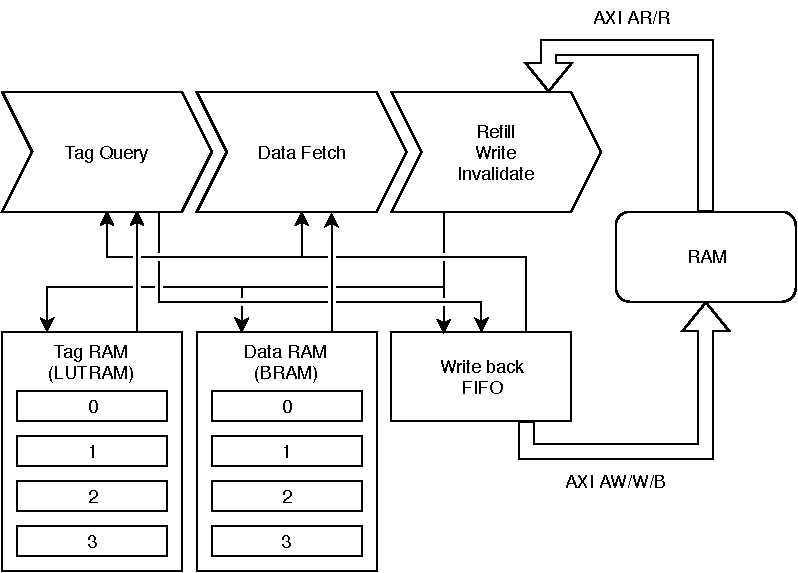
\includegraphics[width=\linewidth]{dcache.pdf}
	\caption{数据缓存结构}
	\label{fig:dcache-structure}
\end{figure}

数据缓存共包含三级流水,结构如图 \ref{fig:dcache-structure} 所示。每一路数据缓存中包含两个 RAM 存储,分别包含每个索引位置的标签和数据。为了能够快速读取,标签存储使用 Xilinx Parameterized Macros 生成的 LUT RAM,可以实现在当前周期读出数据。数据 RAM 使用 Xilinx Parameterized Macros 生成的 Block RAM。

数据缓存还包含一个 FIFO,作为延迟写回的队列。为了实现写合并,FIFO 提供一个额外的随机访问接口,可以使用 FIFO 中某一行的地址完成对于 FIFO 的随机读写。

对于读请求,数据缓存的工作流程如下。
\begin{itemize}
  \item \textbf{第一阶段} 完成对于标签的查询,写回 FIFO 的查询,计算得到缓存命中。
  \item \textbf{第二阶段} 从数据 RAM 中取得对应索引位置的数据,计算读出的数据。
  \item \textbf{第三阶段} 给出数据。如果缓存缺失,通过 AXI 和外设通信,更新缓存,并将覆写位置的脏数据送入 FIFO 中。
\end{itemize}

对于写请求,数据缓存的工作流程如下。
\begin{itemize}
  \item \textbf{第一阶段} 完成对于标签的查询,计算得到缓存命中,完成对于 FIFO 中的写合并操作。
  \item \textbf{第二阶段} 得到数据 RAM 对应索引位置的数据,根据 byteenable 计算得出需要写入数据 RAM 的数据。
  \item \textbf{第三阶段} 完成对标签、数据 RAM 的写入。如果缓存缺失,则进行写分配,并将覆写位置的脏数据送入 FIFO 中。
\end{itemize}

MIPS 要求 CACHE 控制指令必须实现清除、写回特定地址或者索引位置的数据缓存。由于清除也包含写回操作,所以和指令缓存相同,我们实现了清除每一路缓存的特定索引位置,并等待脏数据写回完成。


\section{外部接口}

CPU 整体的结构如图 \ref{fig:cpu-interface} 所示,NonTrivialMIPS CPU 本身暴露三个 AXI 4 Master 接口,分别进行指令读取、数据存取和不过缓存的数据存取。Cache 控制器与 CPU 之间使用自定义的总线信号进行握手和数据传输,以避免在内部使用 AXI 协议带来的不必要延时;而对外,则将必要的访存转换为符合 AXI 规范的信号,与 SoC 进行交互。

由于预赛 \texttt{myCPU} 目录中的 CPU 顶层模块对外只允许暴露一个 AXI 3 Master 接口,我们使用 Xilinx 的 AXI Crossbar IP 将其转换为三个 AXI 4 Slave 接口以适应 CPU 的需要。为了不使得指令预取阻塞访存,crossbar 上的仲裁顺序为 Passthrough > Data Cache > Instruction Cache。在CPU 直接连接到我们设计的 SoC 时,则不使用这一 crossbar,而是将三个 AXI 4 Master 接口直接连接到 Interconnect 上。

\begin{figure}[htbp]
	\centering
	\includegraphics[width=\linewidth]{cpu-interface.pdf}
	\caption{CPU 整体接口架构}
	\label{fig:cpu-interface}
\end{figure}

	